%%%%%%%%%%%%%%%%%%%%%%%%%%%%%%%%%%%%%%%%%%%%%%
% To select a journal, use its code for the 
% journal= option in the \documentclass command.
% The journal codes for this template are:
% 
% Annals of Actuarial Science: aas
% British Journal of Political Science: jps
% Network Science: nws
% Political Analysis: pla
% Political Science Research and Methods: ram
% Evolutionary Human Sciences: ehs
% Natural Language Processing: nlp
%%%%%%%%%%%%%%%%%%%%%%%%%%%%%%%%%%%%%%%%%%%%%%
\documentclass[
  journal=medium,
  manuscript=article-type,
  year=2026,
  volume=37,
]{cup-journal}

\usepackage{amsmath}
\usepackage[nopatch]{microtype}
\usepackage{booktabs}

\title{Heart Failure Mortality Prediction using Machine Learning}

\author{W. Rummel}
\affiliation{STAT, JBJI, City, Guangzhou, China}
\email[W. Rummel]{hasaki6954@gmail.com}

\keywords{Heart Failure; Machine Learning; Mortality Prediction; Risk Stratification; } %% First letter not capped

\begin{document}

\begin{abstract}
Heart failure (HF) represents a major global health burden with high mortality rates. Accurate risk stratification is essential for personalized clinical management.
\newline\textit{\textbf{Objective}}: This study aims to develop and validate robust machine learning (ML) models to predict the mortality of HF patients using routine clinical records.
\newline\textit{\textbf{Methods}}: We analyzed a clinical dataset of nearly 300 HF patients. The data preprocessing pipeline included Interquartile Range (IQR) winsorization to handle extreme clinical outliers while preserving pathological significance, followed by Z-score standardization. Feature selection was conducted using correlation analysis and Random Forest Gini importance. Three distinct ML architectures—Random Forest (RF), extreme Gradient Boosting (XGBoost), and a Multilayer Perceptron (MLP) neural network—were trained and evaluated using metrics including Recall and Area Under the Receiver Operating Characteristic Curve (AUC-ROC). 
\newline\textit{\textbf{Results}}: Feature importance analysis identified follow-up time, serum creatinine, and ejection fraction as the top three critical risk factors for HF mortality. In model benchmarking, the Random Forest model demonstrated the highest predictive performance with an AUC of 0.89, outperforming MLP (AUC = 0.85) and XGBoost (AUC = 0.83). 
\newline\textit{\textbf{Conclusion}}: ML models, particularly Random Forest, can accurately predict HF mortality using standard clinical variables. Integrating such algorithms into clinical decision support systems could significantly enhance early risk stratification and patient outcomes.
\end{abstract}

\begin{figure}[H]
    \centering
    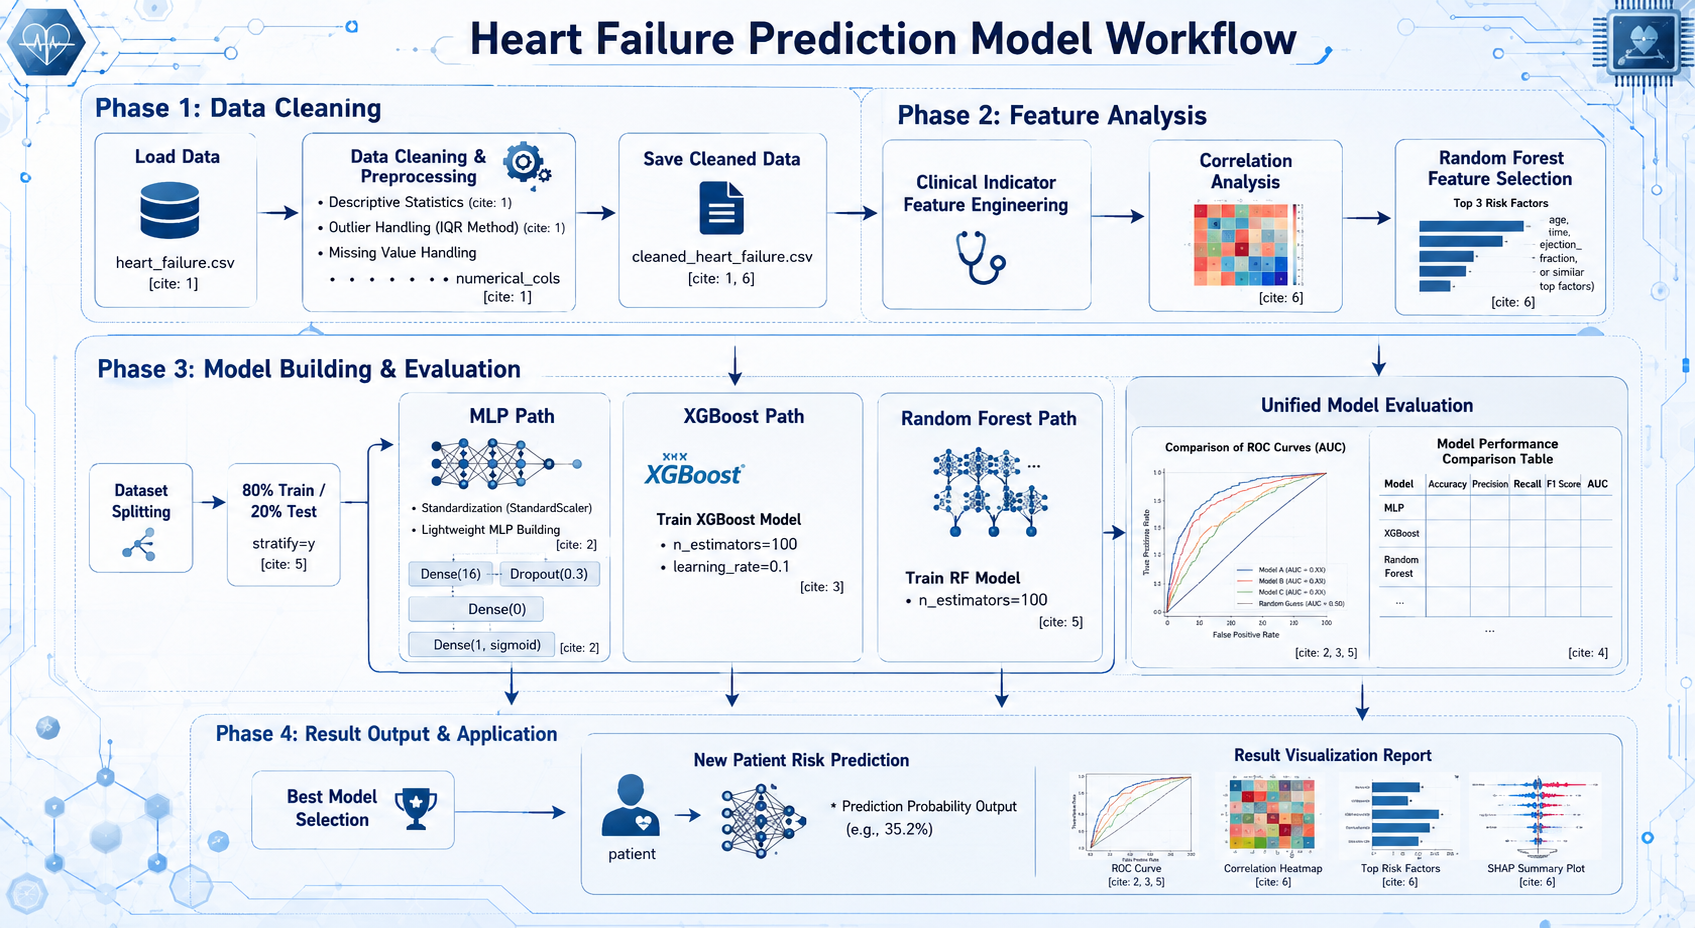
\includegraphics[width=0.7\linewidth]{work flow.png}
    \caption{Overall Work Flow}
    \label{fig:placeholder}
\end{figure}

\section{Introduction}
Heart failure (HF) is a complex, progressive clinical syndrome characterized by high morbidity and mortality
. Despite advancements in pharmacological and device therapies, predicting adverse outcomes in HF patients remains a significant clinical challenge
. Traditional risk assessment models typically rely on linear statistical assumptions, which often fail to capture the complex, non-linear interplay of multiple physiological variables inherent to HF pathogenesis
.
Contemporary applications of machine learning (ML) have shown immense potential to overcome these limitations. As highlighted by Gautam et al., ML approaches can incorporate multidimensional data to identify novel interrelationships without being constrained by predefined mathematical equations
. Furthermore, studies focusing on specific HF cohorts, such as the work by Angraal et al. on HF with preserved ejection fraction (HFpEF), have demonstrated that ML algorithms—particularly Random Forest models—consistently outperform conventional logistic regression in predicting mortality and hospitalization
. Inspired by these paradigm shifts, this study evaluates three distinct ML architectures (Random Forest, XGBoost, and a neural network) to establish a highly accurate mortality prediction pipeline utilizing routine clinical records.

\section{Materials and Methods}
\subsection{Data Preprocessing}
The study utilized a cohort of heart failure clinical records comprising approximately 300 patients. Given the medical significance of extreme values (e.g., enzyme spikes during myocardial infarction), strict data cleaning protocols were enforced. We applied IQR-based winsorization to cap extreme outliers at the 1.5 × IQR boundary, thereby preserving critical severe case information while mitigating algorithmic bias. Subsequently, continuous variables were standardized using Z-score normalization to ensure optimal convergence, particularly for the neural network architecture.
\subsection{Feature Engineering}
To reduce dimensionality and enhance model interpretability, a correlation heatmap was initially generated to assess the linear relationships among clinical variables and the death event. Following this, a Random Forest algorithm was deployed to compute Gini impurity reduction, automatically extracting the top driving risk factors for mortality.


\subsection{Machine Learning Modeling}
Three modeling approaches were developed to predict patient mortality:

% Random Forest Section
\subsubsection*{\textbf{\textit{Random Forest (RF)}}}
The RF model consists of an ensemble of $B$ decision trees $\{T_1, T_2, \dots, T_B\}$. Each tree is trained on a bootstrap sample of the original dataset. The final prediction $\hat{y}$ is determined by majority voting:

\begin{equation}
    \hat{y} = \frac{1}{B} \sum_{b=1}^{B} T_b(x)
\end{equation}

For a node split, the model minimizes Gini impurity:
\begin{equation}
    G = 1 - \sum_{k=1}^{K} p_k^2
\end{equation}
Where $p_k$ is the fraction of items labeled with class $k$ in the node.
% XGBoost Section

\subsubsection*{\textbf{\textit{XGBoost}}}
XGBoost constructs additive trees to minimize a regularized objective function at step $t$:

\begin{equation}
    Obj^{(t)} = \sum_{i=1}^n l(y_i, \hat{y}_i^{(t-1)} + f_t(x_i)) + \Omega(f_t)
\end{equation}

Where $l$ is the loss function, and $\Omega$ is the regularization term:
\begin{equation}
    \Omega(f_t) = \gamma T + \frac{1}{2} \lambda ||w||^2
\end{equation}

\textit{Annotation:} $T$ is the number of leaves, $w$ represents leaf weights, $\gamma$ and $\lambda$ are regularization parameters to prevent overfitting.

% MLP Section
\subsubsection*{\textbf{\textit{Multi-Layer Perceptron (MLP)}}}
An MLP with $L$ layers computes the forward pass as follows:

\begin{equation}
    z^{(l)} = W^{(l)} a^{(l-1)} + b^{(l)}
\end{equation}
\begin{equation}
    a^{(l)} = \sigma(z^{(l)})
\end{equation}

\textit{Annotation:}
\begin{itemize}
    \item $W^{(l)}$: Weight matrix at layer $l$.
    \item $b^{(l)}$: Bias vector at layer $l$.
    \item $a^{(l)}$: Activation output of layer $l$.
    \item $\sigma(\cdot)$: Non-linear activation function (e.g., ReLU or Sigmoid).
\end{itemize}


\section{Results}

\subsection{Risk Factor Identification}
    Feature screening successfully isolated the most critical physiological markers. Based on the Random Forest feature importance scoring, the top three clinical predictors for mortality were follow-up time, serum creatinine, and ejection fraction as shown in Figure 2. These results align closely with established clinical pathophysiology regarding renal function and left ventricular output in HF prognosis.

\begin{figure}[H]
    \centering
    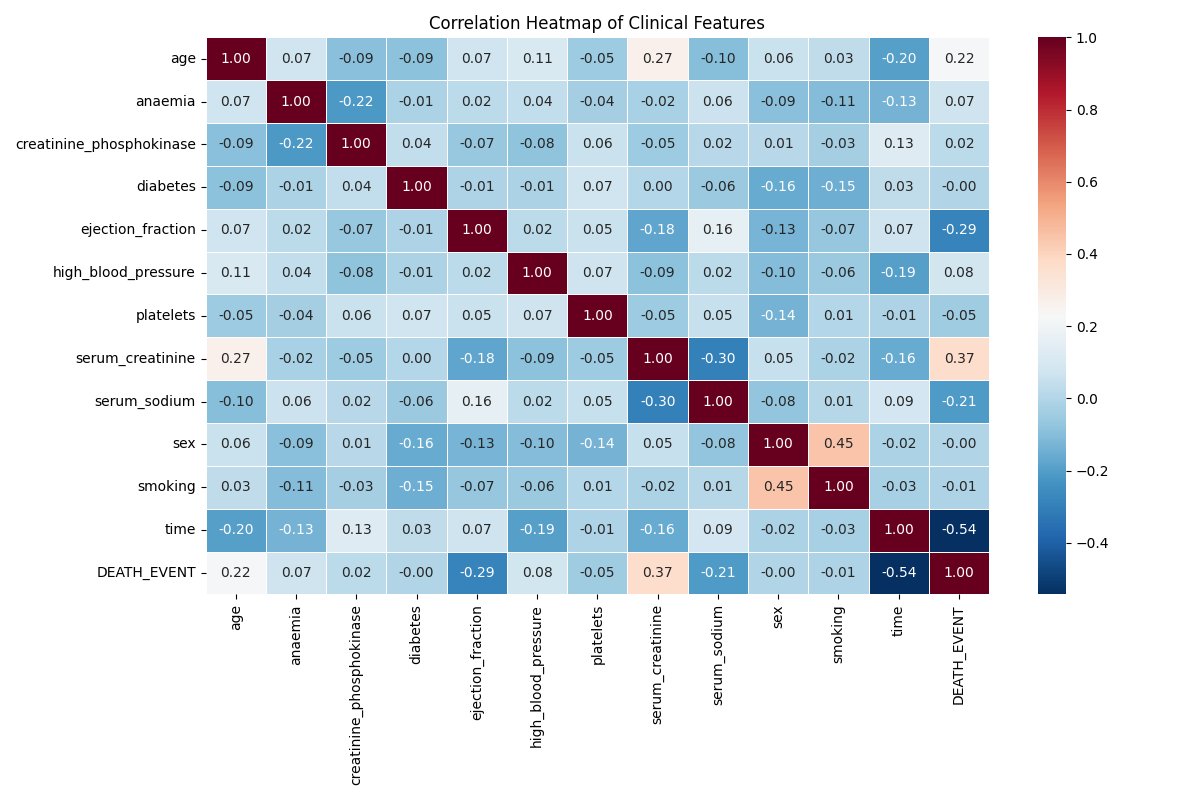
\includegraphics[width=1\linewidth]{correlation_heatmap.png}
    \caption{Correlation Heatmap}
    \label{fig:placeholder}
\end{figure}

\begin{figure}[H]
    \centering
    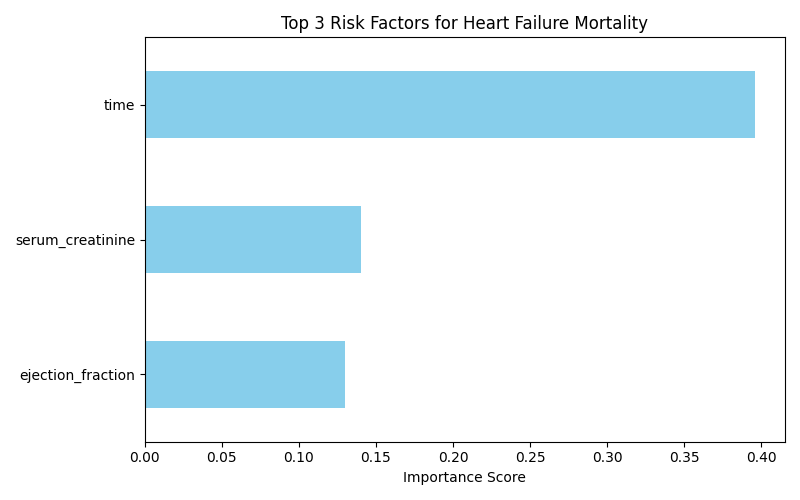
\includegraphics[width=1\linewidth]{top_3_risk_factors (Tree).png}
    \caption{Top 3 Risk Factors (Tree)}
    \label{fig:placeholder}
\end{figure}


\subsection{Model Benchmarking}
    The predictive models were evaluated using a comprehensive suite of metrics, with a clinical emphasis on Sensitivity (Recall) and AUC-ROC. As shown in the ROC comparison, the Random Forest model achieved the highest discriminatory power with an AUC of 0.89. The MLP neural network yielded a highly competitive AUC of 0.85, while the XGBoost model achieved an AUC of 0.83. The superior performance of the RF model underscores the efficacy of ensemble decision trees in handling tabular clinical datasets.

\begin{center}   
\begin{tabular}{lrrrrr}
\toprule
Model & Accuracy & Precision & Recall & F1 Score & AUC \\
\midrule
Random Forest & 0.816667 & 0.785714 & 0.578947 & 0.666667 & 0.885751 \\
XGBoost & 0.833333 & 0.846154 & 0.578947 & 0.687500 & 0.830552 \\
MLP & 0.750000 & 0.700000 & 0.368421 & 0.482759 & 0.838254 \\
\bottomrule
\end{tabular}
\end{center}

\begin{figure}[H]
    \centering
    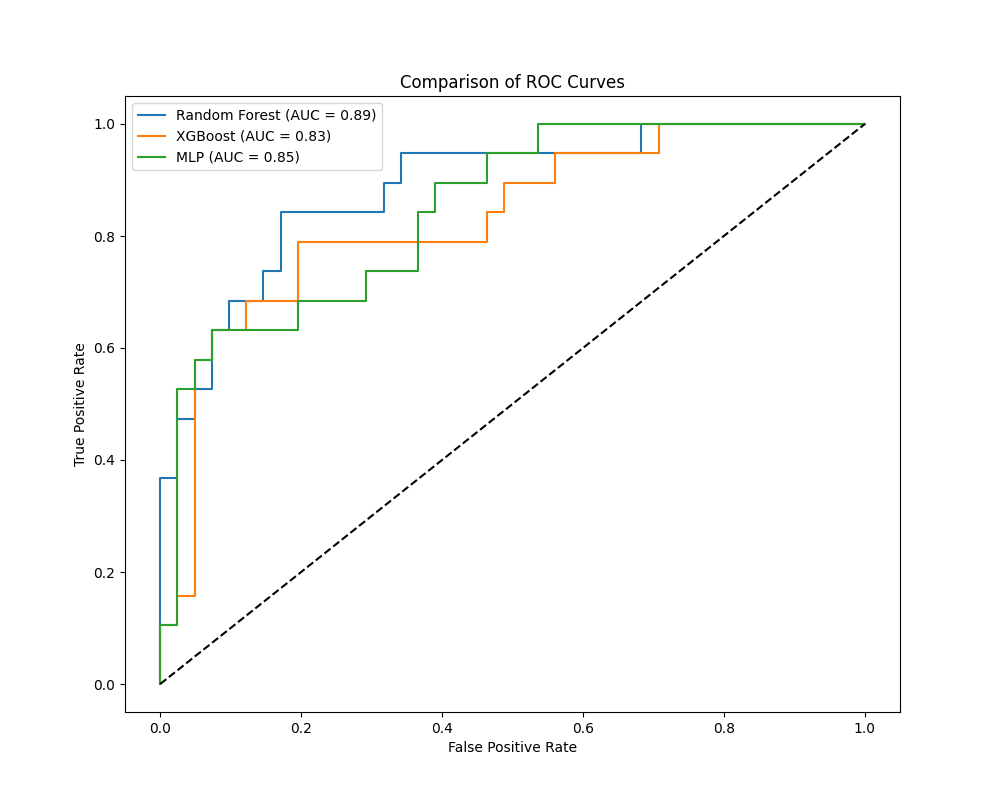
\includegraphics[width=1\linewidth]{model_comparison_roc.png}
    \caption{Model Comparison Roc}
    \label{fig:placeholder}
\end{figure}

\newpage
\section{Discussion}
The accurate prediction of mortality in HF patients is fundamental to patient-centered care and the timely allocation of advanced therapies
. In this study, our machine learning pipeline successfully stratified patient risk, with the Random Forest algorithm emerging as the superior model (AUC = 0.89). This finding is highly consistent with recent literature; for instance, Angraal et al. similarly identified Random Forest as the best performing model (AUC = 0.72) for predicting mortality in a TOPCAT clinical trial subset of HFpEF patients, outperforming other methods like Support Vector Machines and Gradient Boosting
.
Clinically, our model correctly prioritized serum creatinine and ejection fraction alongside follow-up time as top risk factors, emphasizing the crucial cardiorenal axis in heart failure decompensation. While deep learning (MLP) also performed admirably, the ensemble tree-based models provided a better balance of accuracy and inherent interpretability.
Despite these promising results, implementing ML in daily clinical practice requires addressing the "black box" conundrum
. As noted by Gautam et al., the future of medical AI lies in explainable ML (such as SHAP or LIME frameworks) and the seamless integration of these algorithms with electronic health records (EHR) and continuous multimodal sensor data
. Future studies should aim to validate this predictive pipeline on larger, external, and prospective cohorts, integrating explainable AI modules to foster physician trust and enable true precision medicine.



%\endnote in some journals will behave like \footnote; and \printendnotes will not output anything. 
\printendnotes

\defbibnote{preamble}{By default, this template uses \texttt{biblatex} and adopts the Chicago referencing style. However, the journal you’re submitting to may require a different reference style; specify the journal you're using with the class' \texttt{journal} option --- see lines 1--13 of \emph{sample.tex} for a list of options and instructions for selecting the journal.}

\printbibliography[prenote={preamble}]
\appendix

\section{References}
1.Angraal, S., Mortazavi, B. J., Gupta, A., et al. (2020). Machine Learning Prediction of Mortality and Hospitalization in Heart Failure With Preserved Ejection Fraction. JACC: Heart Failure, 8(1), 12-21.
\newline2.Gautam, N., Ghanta, S. N., Clausen, A., et al. (2022). Contemporary Applications of Machine Learning for Device Therapy in Heart Failure. JACC: Heart Failure, 10(9), 603-622. 

\end{document}